% Copyright (c) 2015 Daniele Masini - d.masini.it@gmail.com
% Copyright (c) 2016 Daniele Zambelli - daniele.zambelli@gmail.com

\section{Esercizi}

\subsection{Esercizi dei singoli paragrafi}

\begingroup
\hypersetup{linkcolor=black}
\subsubsection*{\ref{sect:poligoni_equivalenti} - 
\nameref{sect:poligoni_equivalenti}}
\endgroup

\begin{multicols}{2}

\begin{esercizio}
\label{ese:7.1}
Enuncia e dimostra il teorema le cui ipotesi e tesi sono indicate 
di seguito.

\noindent Ipotesi: $AB\parallel DC$, $GH\perp AB$, $CJ\perp AB$, 
$AE\cong DE$, $CF\cong FB$.\\
\noindent Tesi: $ABCD\doteq GHJI$.\\

%
% \begin{inaccessibleblock}[Figura: TODO]
%  \begin{figure}[!htb]
% \noindent\centering% Copyright (c) 2015 Daniele Masini - d.masini.it@gmail.com

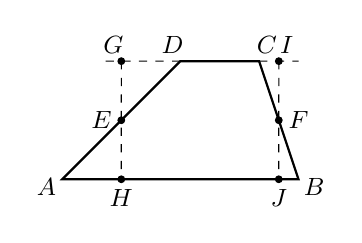
\begin{tikzpicture}[scale=1,font=\small]
\usetikzlibrary{calc}

\begin{scope}
\coordinate (a) at (0,0);
\coordinate (b) at (3,0);
\coordinate (c) at (2.5,1.5);
\coordinate (d) at (1.5,1.5);


\draw[thick] (a) node[shift={(-0.2,-0.1)}] {$A$} -- (b) node[shift={(0.2,-0.1)}] {$B$} -- (c) node[shift={(0.1,0.2)}] {$C$} -- (d) node[shift={(-0.1,0.2)}] {$D$} -- cycle;


\coordinate (e) at ($(a)!0.5!(d)$);
\coordinate (h) at ($(a)!(e)!(b)$);
\coordinate (f) at ($(b)!0.5!(c)$);
\coordinate (j) at ($(a)!(f)!(b)$);
\coordinate (g) at (intersection of h--e and c--d);
\coordinate (i) at (intersection of j--f and c--d);

\draw[dashed] (d) -- ($(d)!1.3!(g)$);
\draw[dashed] (c) -- ($(c)!2!(i)$);

\draw[dashed] (g) -- (h);
\draw[dashed] (i) -- (j);

\draw[fill] (e) circle (1.2pt) node[left] {$E$};
\draw[fill] (f) circle (1.2pt) node[right] {$F$};
\draw[fill] (g) circle (1.2pt) node[shift={(-0.1,0.2)}] {$G$};
\draw[fill] (i) circle (1.2pt) node[shift={(0.1,0.2)}] {$I$};
\draw[fill] (h) circle (1.2pt) node[below] {$H$};
\draw[fill] (j) circle (1.2pt) node[below] {$J$};

\end{scope}


\end{tikzpicture}

%	\caption{Esercizio~\ref{ese:7.1}}\label{fig:ese7.1}
%\end{figure}
% \end{inaccessibleblock}
\end{esercizio}
 
\begin{esercizio}
\label{ese:7.2}
Dai vertici $B$ e $C$ dell'ipotenusa di un triangolo rettangolo $ABC$ 
traccia le rette rispettivamente parallele ai cateti $AC$ e $AB$; sia 
$D$ il loro punto di intersezione. Dimostrare che $ABDC\doteq 2\cdot 
ABC$ e che $MNPQ\doteq 2\cdot ABC$ dove $MNPQ$ è il rettangolo avente 
un lato congruente all'ipotenusa $BC$ e l'altro lato congruente 
all'altezza $AH$ relativa all'ipotenusa.
\end{esercizio}

\begin{esercizio}
\label{ese:7.3}
Costruire un rettangolo equivalente ad un trapezio dato.
\end{esercizio}

\begin{esercizio}
\label{ese:7.4}
Dimostrare che la mediana relativa ad un lato di un triangolo divide 
il triangolo dato in due triangoli equivalenti.
\end{esercizio}

\begin{esercizio}
\label{ese:7.5}
Dimostrare che in un parallelogramma $ABCD$ sono equivalenti i 
quattro triangoli determinati dalle diagonali $AC$ e $BD$.
\end{esercizio}

\begin{esercizio}
\label{ese:7.6}
Assegnato il trapezio $ABCD$, detto $E$ il punto di intersezione 
delle diagonali $DB$ e $AC$, dimostrare che $DEA$ è equivalente a 
$BEC$.
\end{esercizio}


\end{multicols}

\begingroup
\hypersetup{linkcolor=black}
\subsubsection*{\ref{sect:applicazioni_algebra} - 
\nameref{sect:applicazioni_algebra}}
\endgroup

\begin{multicols}{2}


\begin{esercizio}
\label{ese:7.16}
Due lati consecutivi di un parallelogramma misurano $2a$ e $4a$ e 
l'angolo tra essi compreso misura $60\grado$. Trovare la misura 
dell'area e delle diagonali.
\hfill[$A=4\sqrt{3}a^2$,\quad $d_1=2\sqrt{3}a$,\quad $d_2=2\sqrt{7}a$]
\end{esercizio}

\begin{esercizio}
\label{ese:7.18}
Determinare perimetro ed area di un triangolo isoscele, sapendo che 
la base misura $10a$ e che l'angolo adiacente ad uno degli angoli 
alla base misura $150\grado$.
\hfill[$2p=10a(2\sqrt{3}+3)/3$,\quad $A=25a^2/\sqrt{3}$]
\end{esercizio}


\begin{esercizio}
\label{ese:7.21}
\`E dato un trapezio isoscele avente un angolo di $45\grado$ e il 
lato obliquo che misura 2~cm. Trovare l'area sapendo che la base 
minore misura $\sqrt{3}$~cm.
\hfill[$2+\sqrt{6}$~cm\textsuperscript{2}]
\end{esercizio}

\begin{esercizio}
\label{ese:7.23}
Il quadrato $ABCD$ ha il lato di 2~m; costruite sul lato $DC$ il 
triangolo isoscele $DEC$ di base $DC$ e avente 
$D\widehat{E}C=120\grado$; siano $F$ e $G$ i punti di intersezione 
delle rette $ED$ e $EC$ con la retta $AB$. Determinate la misura dei 
lati del triangolo $EFG$.
\hfill[$4+2/\sqrt{3}$,\quad $4\sqrt{3}+2$]
\end{esercizio}


\begin{esercizio}
\label{ese:7.26}
Nel trapezio rettangolo $ABCD$ di base maggiore $AB$, l'angolo acuto 
di vertice $B$ misura $45\grado$ e l'altezza è di 8~m. Sapendo che la 
base minore è $3/4$ dell'altezza, determinate perimetro e area del 
trapezio.
\hfill[$28+8\sqrt{2}$,\quad $80$]
\end{esercizio}

\begin{esercizio}
\label{ese:7.27}
Nel parallelogramma $ABCD$ la diagonale minore $AC$ è perpendicolare 
al lato $BC$ e forma col lato $AB$ un angolo di $45\grado$. Sapendo 
che $AC=5$~m, calcolate il perimetro e l'area del parallelogramma.
\hfill[$10(1+\sqrt{2})$,\quad $25$]
\end{esercizio}

\begin{esercizio}
\label{ese:7.28}
Il trapezio $ABCD$ di base maggiore $AB$, ha $\widehat{A}=45\grado$ e 
$\widehat{B}=60\grado$; sapendo che la base minore è uguale 
all'altezza che misura 12~cm, determinate perimetro e area del 
trapezio.
\hfill[$24(9+\sqrt{3})$,\quad $36+12\sqrt{2}+12\sqrt{3}$]
\end{esercizio}

\begin{esercizio}
\label{ese:7.30}
Il triangolo isoscele $ABC$ ha l'angolo in $A$ opposto alla base $BC$ 
di $120\grado$ ed è circoscritto ad una circonferenza di raggio 
$OH=\sqrt{6}$~m; calcolate perimetro e area del triangolo dato.
\hfill[$14\sqrt{2}+8\sqrt{6}$,\quad $14\sqrt{3}+24$]
\end{esercizio}

\begin{esercizio}
\label{ese:7.32}
Nel trapezio rettangolo $ABCD$ la base minore è metà dell'altezza. 
Determinate perimetro e area in funzione della misura $x$ della base 
minore nei casi in cui l'angolo acuto del trapezio è di
\begin{enumeratea}
\item $45\grado$;
\item $30\grado$;
\item $60\grado$.
\end{enumeratea}
\hfill[a)~$2p=2x(\sqrt{2}+3)$; $A=4x^2$,\quad b)~$2p=2x(4+\sqrt{3})$; 
$A=2x^2(1+\sqrt{3})$,\quad c)~$2p=2x(2+\sqrt{3})$; 
$A=2x^2(3+\sqrt{3})$]
\end{esercizio}

\begin{esercizio}
\label{ese:7.33}
Il triangolo $ABC$ è rettangolo e l'angolo di vertice $C$ misura 
$30\grado$; detta $AP$ la bisettrice dell'angolo retto, con $P$ su 
$BC$, e sapendo che $\overline{AP}=a$, determinate, in funzione di 
$a$, perimetro e area del triangolo dato.
\hfill[$\frac{11}{6}a\sqrt{2}+a\sqrt{6}$,\quad $\frac{1}{6}a^2(e+2\sqrt{3})$]
\end{esercizio}

\begin{esercizio}
\label{ese:7.34}
Il segmento $AC$ è la diagonale del quadrilatero $ABCD$ avente 
$A\widehat{B}C=C\widehat{A}D=90\grado$ e 
$B\widehat{C}A=A\widehat{D}C=60\grado$. \`E vero che $ABCD$ è un 
trapezio rettangolo? Calcolate perimetro e area del quadrilatero 
sapendo che $\overline{AC}=2a$.
\hfill[$2p=a+3a\sqrt{3}$,\quad $A=\frac{1}{2}a^2\sqrt{3}$]
\end{esercizio}

\begin{esercizio}
\label{ese:7.36}
In un parallelogramma di area 12~m\textsuperscript{2}, le lunghezze 
di due lati consecutivi sono una il doppio dell'altra e uno degli 
angoli interni misura $60\grado$. Determina la lunghezza delle 
diagonali.
\hfill[$2\sqrt[4]{27}$~m]
\end{esercizio}

\begin{esercizio}
\label{ese:7.38}
La base di un rettangolo è più lunga di 8~cm dell'altezza ed è più 
corta di 10~cm della diagonale. Calcola perimetro ed area del 
rettangolo.
\end{esercizio}

\begin{esercizio}
\label{ese:7.39}
In un triangolo equilatero $ABC$ di lato $l$ individua sul lato $AB$ 
un punto $P$ tale che detti $H$ e $K$ i piedi delle perpendicolari 
condotte da $P$ ai lati $AC$ e $BC$ risulti 
$\overline{PH}^2+\overline{PK}^2=\overline{PC}^2+\np{12,67}$
\end{esercizio}

\begin{esercizio}
\label{ese:7.40}
Un triangolo equilatero e un quadrato hanno lo stesso perimetro. 
Quanto vale il rapporto tra le aree delle due figure?
\hfill[$16/9$]
\end{esercizio}

\begin{esercizio}
\label{ese:7.43}
Disegna un rombo con la diagonale minore lunga 6~cm e la diagonale 
maggiore 8~cm. Costruisci su ciascun lato del rombo un quadrato. 
Unisci i vertici liberi dei quadrati formando un ottagono. Calcolane 
l'area. Calcola anche l'area dei quattro triangoli che si sono 
formati. Calcola inoltre la misura degli angoli interni dell'ottagono.
\hfill[12~cm\textsuperscript{2},\quad 12~cm\textsuperscript{2},\quad 
$172\grado$]
\end{esercizio}

\begin{esercizio}
\label{ese:7.44}
Disegna un quadrato $ABCD$ e sul lato $AB$ poni i punti $M$ ed $N$ in 
modo che $AM\cong MN\cong NB$. Che figura è $MNCD$? Calcola il 
rapporto tra l'area di $MNCD$ e quella di $ABCD$. Calcola il 
perimetro di $MNCD$ sapendo che l'area del quadrato è 
10~cm\textsuperscript{2}.
\hfill[$\np{0,665}$,\quad $\np{10,85}$~cm]
\end{esercizio}

\begin{esercizio}
\label{ese:7.45}
Disegna un triangolo isoscele $ABC$ di base $AC=40$~mm e lato obliquo 
$AB=52$~mm. Costruisci sulla base $AC$ il triangolo $ACD$ di area 
doppia di $ABC$ e determina il perimetro del quadrilatero $ABCD$. Di 
che figura si tratta?
\hfill[$\np{300,12}$~mm]
\end{esercizio}

\begin{esercizio}
\label{ese:7.46}
Il parallelogramma $ABCD$ ha la base $AB$ lunga 12~cm e l'altezza di 
6~cm. Disegna su $AB$ un punto $H$ e su $CD$ un punto $K$ tali che 
$DK=BH=3$~cm. Considera i due quadrilateri in cui il parallelogramma 
rimane diviso dal segmento $HK$: che quadrilateri sono? Calcolane 
l'area. Calcola inoltre il rapporto tra l'area di $HBCD$ e quella di 
$ABCD$.
\hfill[36,\quad $\np{0,625}$]
\end{esercizio}

\begin{esercizio}
\label{ese:7.47}
Calcola l'altezza del rombo avente le diagonali di 36~cm e 48~cm. 
Calcola l'area del trapezio equivalente al rombo, sapendo che 
l'altezza del trapezio è di 24~cm e che la base maggiore è il doppio 
di quella minore.
\hfill[]
\end{esercizio}

\begin{esercizio}
\label{ese:7.48}
Il rettangolo $R$ ha base $AB = 9$~cm e l'altezza $BC$ è i $4/3$ di 
$AB$. Calcola il perimetro e l'area di $R$. Disegna il 
parallelogramma $P$ equivalente al rettangolo $R$ e avente la base 
congruente alla diagonale del rettangolo. Calcola l'altezza di $P$.
\hfill[42~cm,\quad 108~cm\textsuperscript{2},\quad $\np{7,2}$~cm]
\end{esercizio}

\begin{esercizio}
\label{ese:7.49}
Calcola l'area del parallelogramma $P$ di base \np{4,5}~cm e altezza 
2~cm e con il lato obliquo che è $5/4$ dell'altezza. Disegna la 
diagonale $AC$ e traccia l'altezza relativa ad $AB$ del triangolo 
$ABC$. Calcola l'area del triangolo $ABC$.
\hfill[$\np{11,25}$~cm\textsuperscript{2},\quad 
$\np{5,625}$~cm\textsuperscript{2}]
\end{esercizio}

\begin{esercizio}
\label{ese:7.51}
Dato il rombo $ABCD$, avente perimetro di 10~cm e la diagonale 
maggiore di 4~cm, calcola la misura della diagonale minore, l'area 
del rombo e la sua altezza. Considera un triangolo isoscele 
equivalente al rombo e avente la sua stessa altezza. Calcolane la 
misura di ciascun lato.
\hfill[3~cm,\quad 6~cm\textsuperscript{2},\quad $\np{2,4}$~cm,\quad 
5~cm,\quad $\np{3,5}$~cm]
\end{esercizio}

\begin{esercizio}
\label{ese:7.58}
La differenza tra le diagonali di un rombo è 7~cm e una è $5/12$ 
dell'altra. Determina l'area di un triangolo isoscele il cui 
perimetro supera di 6~cm quello del rombo e la cui base è 8~cm.
\end{esercizio}

\begin{esercizio}
\label{ese:7.59}
Determinare l'area di un quadrilatero con le diagonali perpendicolari 
sapendo che l'una è $5/8$ dell'altra e che la loro somma è 39~cm.
\hfill[]
\end{esercizio}

\begin{esercizio}
\label{ese:7.60}
Determinare la misura degli angoli di un parallelogramma sapendo che 
uno degli angoli alla base è $2/7$ di quello adiacente.
\end{esercizio}

\begin{esercizio}
\label{ese:7.64}
In un rombo la somma delle diagonali misura 196~cm, un quarto della 
misura della diagonale maggiore supera di 4~cm la misura della 
diagonale minore. Trova perimetro, area e altezza del rombo.
\hfill[328~cm,\quad $\np{2880}$~cm\textsuperscript{2},\quad $\np{35,15}$~cm]
\end{esercizio}

\begin{esercizio}
\label{ese:7.65}
In un trapezio rettangolo l'altezza è quadrupla della base minore e 
il lato obliquo è i $5/4$ dell'altezza. Determina l'area del trapezio 
sapendo che il suo perimetro è 70~cm.
\hfill[250~cm\textsuperscript{2}]
\end{esercizio}

\begin{esercizio}
\label{ese:7.66}
Il perimetro di un trapezio isoscele misura 124~cm e ciascun lato 
obliquo è lungo 30~cm. Determinane l'area e la misura della diagonale 
sapendo che una sua base è $7/25$ dell'altra.
\hfill[768~cm\textsuperscript{2},\quad 40~cm]
\end{esercizio}

\begin{esercizio}
\label{ese:7.67}
Determina l'area di un rettangolo sapendo che la misura della sua 
diagonale supera di 8~cm quella dell'altezza e che la differenza fra 
i $20/41$ della diagonale ed i $2/3$ dell'altezza è uguale ai $14/9$ 
della stessa altezza.
\end{esercizio}

\begin{esercizio}
\label{ese:7.69}
Il perimetro di un rettangolo misura 29~cm ed i $2/11$ della sua 
altezza sono uguali a $1/9$ della base. Trovare l'area del rettangolo.
\hfill[$\np{49,5}$~cm\textsuperscript{2}]
\end{esercizio}

\begin{esercizio}
\label{ese:7.77}
Determina il perimetro di un triangolo rettangolo sapendo che 
l'altezza relativa all'ipotenusa è 8~cm e che la proiezione di un 
cateto sull'ipotenusa è $4/3$ dell'altezza data.
\hfill[40~cm]
\end{esercizio}

\begin{esercizio}
\label{ese:7.78}
Determina la misura delle tre altezze del triangolo che ha i lati di 
20~cm, 40~cm, 30~cm. (Suggerimento: Puoi ricorrere alla formula di 
Erone).
\end{esercizio}

\begin{esercizio}
\label{ese:7.80}
Trova il perimetro di un triangolo isoscele sapendo che la base è 
$2/3$ dell'altezza e che l'area è 24~cm\textsuperscript{2}.
\end{esercizio}

\begin{esercizio}
\label{ese:7.81}
Trova il perimetro di un triangolo isoscele sapendo che la base è 
$3/5$ dell'altezza e che l'area è 24~cm\textsuperscript{2}.
\end{esercizio}

\begin{esercizio}
\label{ese:7.82}
I lati del triangolo $ABC$ hanno le misure seguenti $AB=63$~cm, 
$BC=60$~cm e $AC=39$~cm; determina le misure delle tre relative 
altezze.
\end{esercizio}

\begin{esercizio}
\label{ese:7.83}
Determinare la misura di ciascun lato e l'area del triangolo isoscele 
avente il perimetro di 700~m, sapendo che la base e il lato obliquo 
sono in rapporto $\frac{16}{17}$.
\hfill[224~m,\quad 238~m,\quad $\np{23520}$~m\textsuperscript{2}]
\end{esercizio}

\begin{esercizio}
\label{ese:7.87}
In un trapezio rettangolo, l'angolo che il lato obliquo forma con la 
base maggiore ha ampiezza $60\grado$ e la diagonale maggiore dimezza 
tale angolo; sapendo che la base minore misura 4~cm,  calcolare il 
perimetro del trapezio.
\hfill[$14 + 2\sqrt{3}$~cm]
\end{esercizio}

\begin{esercizio}
\label{ese:7.91}
Determina area e perimetro del quadrilatero $ABCD$ di coordinate 
$A(-1;7)$, $B(6;9/2)$, $C(4;-3)$ e $D(-4;3)$.
\hfill[$\np{30,2}$,\quad $\np{53,75}$]
\end{esercizio}

\begin{esercizio}
\label{ese:7.92}
Determina area a perimetro del quadrilatero $ABCD$ di coordinate 
$A(0;3)$, $B(3;6)$, $C(6;3)$ e $D(-4;3)$. Che quadrilatero è?
\hfill[$\np{22,4}$; $\np{19,5}$]
\end{esercizio}

\begin{esercizio}
\label{ese:7.93}
Determina l'area del quadrilatero $ABCD$ di coordinate $A(-8;5)$, 
$B(-2;11)$, $C(2;12)$ e $D(4;3)$.
\hfill[$A=14$]
\end{esercizio}

\begin{esercizio}
\label{ese:7.94}
Determina il quarto vertice $D$ del trapezio $ABCD$ di area $9$, 
sapendo che $A(-1;2)$, $B(5;2)$ e $C(3;4)$.
\end{esercizio}

\begin{esercizio}
\label{ese:7.95}
Determina il quarto vertice $D$ del parallelogramma $ABCD$ con 
$A(-3;-1)$, $B(4;1)$ e $C(3;4)$.
\hfill[$D(-4;2)$]
\end{esercizio}

\begin{esercizio}
\label{ese:7.96}
Verifica che il trapezio di vertici $A(-1;-1)$, $B(3;-2)$, 
$C\left(3;\frac{1}{2}\right)$ e $D\left(0;\frac{5}{2}\right)$ non è 
rettangolo. Calcola l'intersezione $E$ dei prolungamenti dei lati 
obliqui $BC$ e $AD$. Calcola inoltre il rapporto tra le aree dei 
triangoli $ABE$ e $CDE$.
\end{esercizio}

\begin{esercizio}
\label{ese:7.97}
Verifica che il quadrilatero di vertici $A(-2;-3)$, $B(3;-2)$, 
$C(4;1)$ e $D(0;3)$ è un trapezio e calcolane l'altezza.
\end{esercizio}

\begin{esercizio}
\label{ese:7.98}
Verifica che il quadrilatero di vertici $A(-4;1)$, $B(5;-2)$, 
$C(3;2)$ e $D(0;3)$ è un trapezio isoscele. Calcola l'intersezione $E$ 
dei prolungamenti dei lati obliqui $BC$ e $AD$. Calcola inoltre il 
rapporto tra le aree dei triangoli $ABE$ e $CDE$.
\end{esercizio}

\begin{esercizio}[Giochi di Archimede 2007]
\label{ese:7.104}
$ABCD$ è un quadrato avente la diagonale lunga 2~cm e $AEC$ è 
equilatero. Quanto vale l'area del quadrilatero $AECB$?
\end{esercizio}

%
% \begin{inaccessibleblock}[Figura: TODO]
%  \begin{figure}[!htb]
% 	\centering% Copyright (c) 2015 Daniele Masini - d.masini.it@gmail.com

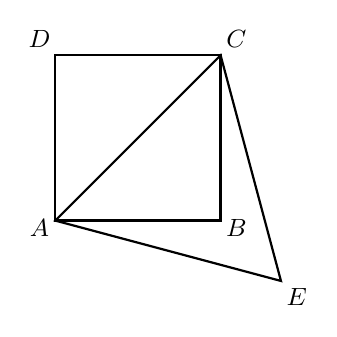
\begin{tikzpicture}[scale=0.7,font=\small]
\usetikzlibrary{calc, intersections}

\begin{scope}
\clip (-0.5,-1.6) rectangle (4.6,3.5);
\coordinate (a) at (0,0);
\coordinate (b) at (3,0);
\coordinate (c) at (3,3);
\coordinate (d) at (0,3);

\path[name path = Circle1] (a) let \p1 = ($(c)-(a)$) in circle ({veclen(\x1,\y1)});
\path[name path = Circle2] (c) let \p1 = ($(a)-(c)$) in circle ({veclen(\x1,\y1)});
\path [name intersections={of=Circle1 and Circle2}];
\path (intersection-2) coordinate (e) node[shift={(0.2,-0.2)}] {$E$};

\draw[thick] (a) node[shift={(-0.2,-0.1)}] {$A$} -- (b) node[shift={(0.2,-0.1)}] {$B$} -- (c) node[shift={(0.2,0.2)}] {$C$} -- (d) node[shift={(-0.2,0.2)}] {$D$} -- cycle;
\draw[thick] (a) -- (c) -- (e) -- cycle;

\end{scope}


\end{tikzpicture}

%	\caption{Esercizio~\ref{ese:7.105}}\label{fig:ese7.105}
%\end{figure}
% \end{inaccessibleblock}
%
% \begin{inaccessibleblock}[Figura: TODO]
%  \begin{figure}[!htb]
% 	\centering% Copyright (c) 2015 Daniele Masini - d.masini.it@gmail.com

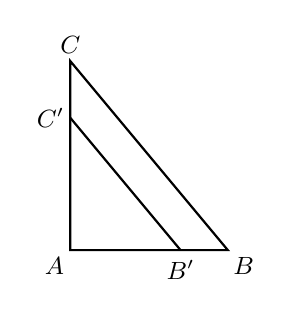
\begin{tikzpicture}[scale=0.8,font=\small]
\usetikzlibrary{calc}

\begin{scope}
%\clip (-2.1,-2.1) rectangle (2.5,2.1);
\coordinate (a) at (0,0);
\coordinate (b) at (2.5,0);
\coordinate (c) at (0,3);

\draw[thick] (a) node[shift={(-0.2,-0.2)}] {$A$} -- (b) node[shift={(0.2,-0.2)}] {$B$} -- (c) node[shift={(0,0.2)}] {$C$} -- cycle;

\draw[thick] ($(a)!0.7!(b)$) node[shift={(0,-0.25)}] {$B'$} -- ($(a)!0.7!(c)$) node[shift={(-0.25,0)}] {$C'$};

\end{scope}


\end{tikzpicture}

%	\caption{Esercizio~\ref{ese:7.108}}\label{fig:ese7.108}
%\end{figure}
% \end{inaccessibleblock}


\begin{esercizio}[Giochi d'Autunno 2011]
\label{ese:7.109}
Nel parallelogramma $ABCD$ il segmento $BD$ è perpendicolare ad $AB$ 
ed $E$ e $F$ sono i punti medi di $AB$ e $CD$ rispettivamente. 
Calcolare l'area del quadrilatero $GEHF$, sapendo che $AB=5$~cm e 
$BD=2$~cm.
\end{esercizio}

%
% \begin{inaccessibleblock}[Figura: TODO]
%  \begin{figure}[!htb]
% 	\centering% Copyright (c) 2015 Daniele Masini - d.masini.it@gmail.com

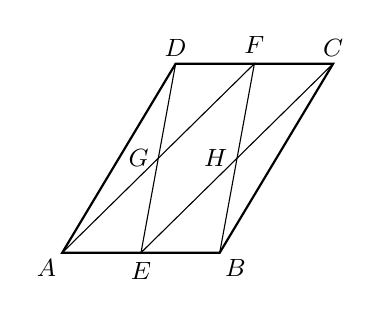
\begin{tikzpicture}[scale=0.8,font=\small]
\usetikzlibrary{calc}

\begin{scope}
\coordinate (a) at (0,0);
\coordinate (b) at (2.5,0);
\coordinate (c) at (4.3,3);
\coordinate (d) at (1.8,3);
\coordinate (e) at ($(a)!0.5!(b)$);
\coordinate (f) at ($(c)!0.5!(d)$);

\draw[thick] (a) node[shift={(-0.2,-0.2)}] {$A$} -- (b) node[shift={(0.2,-0.2)}] {$B$} -- (c) node[shift={(0,0.2)}] {$C$} -- (d) node[shift={(0,0.2)}] {$D$} -- cycle;

\draw (a) -- (f) -- (b);
\draw (c) -- (e) -- (d);

\coordinate (h) at (intersection of e--c and f--b);
\coordinate (g) at (intersection of d--e and a--f);

\node[above] at (f) {$F$};
\node[below] at (e) {$E$};

\node[left] at (g) {$G$};
\node[left] at (h) {$H$};

\end{scope}


\end{tikzpicture}

%	\caption{Esercizio~\ref{ese:7.110}}\label{fig:ese7.110}
%\end{figure}
% \end{inaccessibleblock}

\begin{esercizio}[Giochi d'Autunno 2010]
\label{ese:7.110}
In un triangolo due angoli misurano rispettivamente $30\grado$ e 
$105\grado$ ed il lato tra essi compreso è lungo 2~cm. Qual è la 
misura del perimetro del triangolo? 
\end{esercizio}

\begin{esercizio}[Giochi d'Autunno 2011]
\label{ese:7.111}
In un parallelogramma di area 1~m\textsuperscript{2} le lunghezze di 
due lati consecutivi sono una il doppio dell'altra. Inoltre uno degli 
angoli interni misura $60\grado$. Quanto misura la diagonale minore?
\end{esercizio}

\begin{esercizio}[Giochi d'Autunno 2010]
\label{ese:7.112}
In un triangolo equilatero $ABC$ con lato di lunghezza 3~m, prendiamo 
i punti $D$, $E$ e $F$ sui lati $AC$, $AB$ e $BC$ rispettivamente, in 
modo che i segmenti $AD$ e $FC$ misurino 1~m e il segmento $DE$ sia 
perpendicolare ad $AC$. Quanto misura l'area del triangolo $DEF$?
\end{esercizio}

%
% \begin{inaccessibleblock}[Figura: TODO]
%  \begin{figure}[!htb]
% 	\centering% Copyright (c) 2015 Daniele Masini - d.masini.it@gmail.com

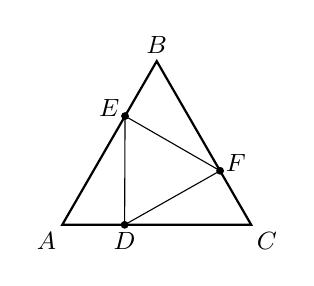
\begin{tikzpicture}[scale=1.2,font=\small]
\usetikzlibrary{calc}

\begin{scope}
\draw[thick] (0,0) coordinate (a) node[shift={(-0.2,-0.2)}] {$A$} -- ++(0:2) coordinate (c) node[shift={(0.2,-0.2)}] {$C$} -- ++(120:2) coordinate (b) node[shift={(0,0.2)}] {$B$} -- cycle;

\coordinate (d) at ($(a)!0.33!(c)$);
\coordinate (f) at ($(c)!0.33!(b)$);
\path (d) let \p1 = (d) in -- ({\x1},{\y1+1}) coordinate (d1);
\coordinate (e) at (intersection of d--d1 and a--b);

\draw (d) -- (e) -- (f) -- cycle;

\draw[fill] (d) circle (1pt) node[shift={(0,-0.2)}] {$D$};
\draw[fill] (e) circle (1pt) node[shift={(-0.2,0.1)}] {$E$};
\draw[fill] (f) circle (1pt) node[shift={(0.2,0.1)}] {$F$};

\end{scope}


\end{tikzpicture}

%	\caption{Esercizio~\ref{ese:7.113}}\label{fig:ese7.113}
%\end{figure}
% \end{inaccessibleblock}

\begin{esercizio}[Giochi di Archimede 2005]
\label{ese:7.113}
Dato un quadrato $ABCD$ si uniscono i punti medi dei lati aventi un 
vertice in comune formando un nuovo quadrato $EFGH$. Ripetiamo la 
stessa operazione per $EFGH$ e otteniamo un nuovo quadrato 
$A'B'C'D'$. Quanto vale il rapporto tra l'area di $ABCD$ e l'area di 
$A'B'C'D'$?
\end{esercizio}

\end{multicols}

